% SZABLON PRACY MAGISTERSKIEJ - WERSJA 1.0 Z 14 LUTEGO 2010 - MARCIN KULCZYCKI
% Szablon wymaga LaTeXa z zainstalowanymi polskimi stylami
% W skład szablonu wchodzą pliki szablon_mgr.tex i logo_uj.png
% Plik należy kompilować bezpośrednio do formatu .pdf, nie do .dvi (inaczej grafika nie złoży się dobrze)

% Uwaga! Po każdej większej zmianie oraz przed ostatecznym drukiem plik należy przeLaTeXować trzy razy pod
% rząd, aby referencje, cytowania oraz spis treści miały szansę złożyć się we właściwy sposób.

\documentclass[12pt,a4paper,oneside]{amsbook}

\usepackage[utf8]{inputenc}
\usepackage{amssymb} % To pakiet z dodatkowymi symbolami matematycznymi
\usepackage{polski} % Te pakiety umożliwiają składanie pracy w języku polskim
\usepackage{graphicx} % Ten pakiet umożliwia umieszczanie obrazków w tekście
\usepackage{indentfirst}	
\usepackage{subfigure}
\usepackage{hyperref}
\usepackage{enumitem}
\usepackage{listings}
\usepackage{anysize}
\usepackage{setspace}

%marginesy
	\marginsize{3.5cm}{2.5cm}{2.5cm}{2.5cm}

	\numberwithin{figure}{section}  % numerowanie obrazków, prefiksowane numerem sekcji
	\numberwithin{table}{section}   % numerowanie tabel, prefiksowane numerem sekcji

%interlinia
	\doublespacing
	
%ustawienia linków (brak obramowania)
	\hypersetup{
	pdfborder={0 0 0 0} 
	}

%brak dzielenia wyrazów
%	\selecthyphenation{nohyphenation}
%	\sloppy

%ustawienia listingów
\lstset{ %
language=XML,                % choose the language of the code
basicstyle=\footnotesize,       % the size of the fonts that are used for the code
numbers=left,                   % where to put the line-numbers
numberstyle=\footnotesize,      % the size of the fonts that are used for the line-numbers
stepnumber=1,                   % the step between two line-numbers. If it's 1 each line will be numbered
numbersep=5pt,                  % how far the line-numbers are from the code
showspaces=false,               % show spaces adding particular underscores
showstringspaces=false,         % underline spaces within strings
showtabs=false,                 % show tabs within strings adding particular underscores
tabsize=2,	                % sets default tabsize to 2 spaces
captionpos=b,                   % sets the caption-position to bottom
breaklines=true,                % sets automatic line breaking
breakatwhitespace=false,        % sets if automatic breaks should only happen at whitespace
title=\lstname,                 % show the filename of files included with \lstinputlisting; also try caption instead of title
escapeinside={\%*}{*)}          % if you want to add a comment within your code
}

\begin{document}

% Strona tytułowa
\begin{center}
\thispagestyle{empty} % Na stronie tytułowej nie chcemy numeru strony

\includegraphics[width=1.5cm, height=1.5cm]{logo_uj.png} % Ta komenda umieszcza na stronie logo UJ

{\large UNIWERSYTET JAGIELLOŃSKI

WYDZIAŁ FIZYKI, ASTRONOMII I INFORMATYKI STOSOWANEJ} \vfill\vfill\vfill\vfill

{\large TOMASZ BOROWSKI \bigskip}

{\Huge SZTUCZNA INTELIGENCJA
W~SYMULATORZE DZIAŁAŃ
ANTYTERRORYSTYCZNYCH}\bigskip\bigskip

{\large PRACA MAGISTERSKA NAPISANA POD KIERUNKIEM

DR HAB. PIOTRA BIAŁASA \vfill\vfill\vfill

KRAKÓW 2012} 
\end{center}


% Streszczenie
\chapter*{Streszczenie}
Niniejsza praca dyplomowa omawia projekt gry symulacyjnej, w~której gracz ma możliwość planowania i przeprowadzania działań antyterrorystycznych. Zastosowane w projekcie algorytmy sztucznej inteligencji, typowe dla gier wideo, zostały uzupełnione algorytmami realizującymi charakterystyczne dla strony konfliktu taktyki. Dokumentacja projektu jest uzupełniona opisem technologi HTML5 Canvas oraz bibliotek JavaScript wykorzystach podczas implementacji.


% Spis treści
\tableofcontents % Spis treści jest generowany automatycznie przez LaTeXa
\let\cleardoublepage\clearpage % To taka mała sztuczka, która nie pozwala LaTeXowi wstawiać pustych stron przed nowymi rozdziałami
\pagestyle{plain} % Ta komenda pozwala pozbyć się nagłówków stron

% Oświadczenie
\chapter*{Oświadczenie}
Świadomy odpowiedzialności prawnej oświadczam, że złożona praca magisterska pt.: „Sztuczna inteligencja w symulatorze działań antyterrorystycznych” została napisana przeze mnie samodzielnie.

Równocześnie oświadczam, że praca ta nie narusza prawa autorskiego w rozumieniu ustawy z dnia 4 lutego 1994 roku o prawie autorskim i prawach pokrewnych (Dz.U.1994 nr 24 poz. 83) oraz dóbr osobistych chronionych prawem cywilnym.

Ponadto praca nie zawiera informacji i danych uzyskanych w sposób nielegalny i~nie była wcześniej przedmiotem innych procedur urzędowych związanych z uzyskaniem dyplomów lub tytułów zawodowych uczelni wyższej.



% Wstęp 
\chapter*{Wprowadzenie}
Gry wideo, które dotychczas kojarzone były niemal wyłącznie z pojęciem interaktywnej formy dostarczania rozrywki, od wielu lat zdobywają coraz to nowsze pola zastosowań. Przykładem tutaj mogą być gry oparte o zasadę tzw. \emph{edutainment} (w~tłum. \emph{edurozrywka})\footnote{przykładowy serwis z grami edukacyjnymi - http://www.edugames.pl/}. Mają one na celu efektywne przekazywanie wiedzy, dzięki swojemu atrakcyjnemu i rozrywkowemu charakterowi, w takich dyscypliach naukowych jak biologia, fizyka, informatyka lub języki obce. 
Innym polem zastosowań elementów gier jest biznes. Coraz częściej można spotkać się z pojęciem \emph{gamefication} (w tłum. \emph{grywalizacji}) miejsca pracy. Określa ono zestaw technik i narzędzi związanych z grami, które pomagają motywować pracowników do lepszego wykonywania powierzonej im pracy. Dzieje się to poprzez nagradzanie najlepszych pracowników wirtualnymi punktami doświadczenia, osiągnięciami oraz umieszczaniem ich wizerunku na szczytach rankingów\footnote{przykładowa aplikacja bazująca na idei grywalizacji - https://dueprops.com/}.
Wreszcie, możemy mieć również do czynienia z~grami symulacyjnymi. Ich celem jest umożliwienie graczom doznawania wrażeń znanych z~rzeczywistości, a których oni bezpośrednio mogą na codzień nie doświadczać. Wśród takich gier można wyróżnić gry, których celem jest szkolenie użytkowników - np. symulatory lotu - oraz te, których głównym celem jest dostarczenie użytkownikom rozrywki - np. symulator prowadzenia sieci pizzerii.

\begin{figure}
\begin{center}
	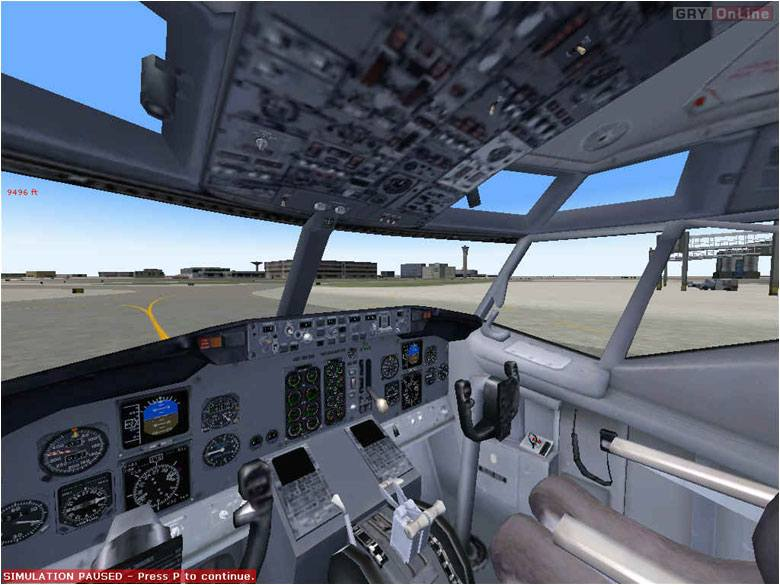
\includegraphics[width=120mm,height=90mm]{images/flightSim}
	\caption{Fligt Simulator 2004 - przykład gry symulacyjnej}
\end{center}
\end{figure}

Niniejsza praca dyplomowa skupia się na projekcie gry symulacyjnej, która odwzorowuje, w dużym uproszczeniu, działania oddziałów antyterrorystyczych podczas szturmu na budynek, zajęty przez wrogie jednostki. Użytkownik grający w tą grę ma możliwość stworzenia schematu budynku, parametryzacji liczby jednostek po obu stronach konfliktu oraz określenia planu działania antyterrorystów. Na podstawie tej konfiguracji gra przeprowadza symulację szturmu na budynek, którą gracz może obserwować.

Realizacja tego projektu obejmuje zaprojektowanie i zaimplementowanie gry oraz omówienie taktyk stosowanych przez strony konfliktu. Zwrócona jest szczególna uwaga na twórcze wykorzystaie algorytmów sztucznej inteligencji, charakterystycznych dla gier wideo. Uzupełnieniem dokumentu jest przedstawienie technologii i bibliotek, które zostały wykorzystane podczas implementacji.




% Wstęp 
\chapter{State of Art}
\section{Planowanie operacji antyterrorystycznych w~rzeczywistości}
Problem terroryzmu i skutków, jakie może on wyrządzać ludności, jest dla instytucji państwowych podstawą do przygotowywania długoterminowych strategii jego zapobiegania. Strategie te ujęte są w dokumentach\footnote{polskim przykładem jest dokument "Narodowy Program Antyterrorystyczny RP na lata 2012-2016"} przygotowywanych przez instrumenty państwowe. Opisują one środki i metody zabezpieczania obywateli przed aktami terroryzmu. Niestety, w zetknięciu z rzeczywistością bywają one nie zawsze skuteczne.

Mając do czynienia z aktem terroryzmu, polegającym na przejęciu kontroli przez terrorystów nad pewną przestrzenią (np. nad budynkiem), służby odpowiadające za bezpieczeństwo podejmują szereg działań, które mają na celu zminimalizować ryzyko utraty zdrowia lub życia przez osoby postronne (w tym ew. zakładników). Prócz zabezpieczenia okolicznego terenu (odizolowaniu go od cywili oraz mediów) oraz prowadzenia negocjacji z terrorystami, bardzo ważnym elementem jest przygotowanie planu przejęcia zakładników oraz ew. eliminacji terrorystów z użyciem siły. Do takiej czynności może dojść w przypadku, gdy terroryści odmówią negocjacji, bądź gdy zaczynają zabijać zakładników.

Proces planowania akcji antyterrorystycznych jest często charakterystyczy dla przeprowadzającej go jednostki specjalnej i zawsze jest strzeżony tajemnicą. Jednakże na przełomie kwietnia i maja 1980 roku, gdy grupa sześciu terrorystów przejęła kontrolę nad Ambasadą Irańską w Londynie, biorąc za zakładników 26 osób, to brytyjskie jednostki specjalne przeprowadziły skuteczną eliminację terrorystów na oczach całego świata\footnote{świadkami operacji byli dziennikarze wielu stacji telewizyjnych, a wśród zakładników byli m.in. reporterzy BBC}. Dzisiaj Operacja Nimrod jest szczegółowo udokumenotwana licznymi artykułami\footnote{przy przygotowywaniu tej pracy został wykorzystany artykuł ze strony Elite UK Forces\cite{eliteUK}}, książkami oraz dokumentami wideo. Dzięki tej wiedzy jesteśmy w stanie odtworzyć proces planowania takiej akcji antyterrorystycznej, co zostało ukazane w tabeli \ref{realPlan}. Spełnienie wszystkich wymienionych czynności znacznie zwiększa szanse na powodzenie operacji: uratowanie zakładników, eliminacja terrorystów i nieodniesienie strat własnych przez jednostkę przeprowadzającą atak.

\begin{table}
\begin{center}
\begin{tabular}{p{0.5\textwidth} p{0.5\textwidth}}
Planowana czynność & Realizacja (Nimrod)\\\hline
	\begin{enumerate}
		\setlength\itemsep{0pt}
		\item Przygotowanie IA Plan\footnote{Immediate Action Plan - plan eliminacji terrorystów, który jest przygotowywany przed powstaniem docelowego planu (najczęściej w tym czasie nie ma jeszcze danych wywiadowczych)}
		\item Zbieranie danych
		\item Rozpoznanie wroga
		\item Rozpoznanie wyposażenia wroga
		\item Rozpoznanie terenu
		\item Określenie niezbędnych środków 
		\item Określenie punktów wejścia
		\item Określenie punktów ewakuacji		
	\end{enumerate}&\begin{enumerate}
		\setlength\itemsep{0pt}
		\item Szturm ambasady od głównego wejścia i zabezpieczanie budynku piętro po piętrze
		\item Zainstalowane podsłuchy w ścianach, snajperzy jako obserwatorzy, sprawdzanie punktów wejścia pod osłoną nocy
		\item Wywiad dostarcza dane osobowe terrorystów, którzy starali się o~wizy w ambasadzie Wielkiej Brytanii w Belgradzie
		\item Jeden z uwolnionych zakładników informuje policję o liczbie i uzbrojeniu terrorystów
		\item Analizowane są plany architektoniczne budynku i prowadzona jest konsultacja z woźnym ambasady
		\item Cztery drużyny (24 żołnierzy), pistolety maszynowe MP5, ładunki wybuchowe, granaty ogłuszające, liny itp.
		\item Wejście przez dach, wejście przez balkony na pierwszym piętrze, wejście tylnymi drzwiami na parterze
		\item Ewakuacja zakładników do ogrodu za budynkiem ambasady
	\end{enumerate}
\end{tabular}
\caption {Czynności dokonywane podczas planowania operacji antyterrorystycznej\label{realPlan}}
\end{center}
\end{table} 

W grze symulacyjnej, będącej przedmiotem tej pracy dyplomowej, gracz może zaplanować podstawowe elementy operacji antyterrorystycznej:
\begin{enumerate}
	\item zdefiniować liczbę terrorystów i antyterrorystów
	\item zaplanować jednopoziomową architekturę budynku
	\item oznaczyć punkty kluczowe wokół których można spodziewać się obecności terrorystów
	\item zdefiniować punkt wejścia oraz punkt ewakuacji
\end{enumerate}

\section{Gry symulacyjne}
Gatunek gier symulacyjnych charakteryzuje się wiernym odzwieciedlaniem realiów świata rzeczywistego lub fikcyjnego. Prócz zastosowania rozrywkowego, gry symulacyjne wykorzystuje się do celów szkoleniowych (np. wirualna nauka jazdy) lub badawczych (np. analiza bezpieczeństwa terytorialnego). Wśród symulacyjnych gier wideo należy wymieć kilka podgatunków\footnote{przedstawiona lista wywodzi się z podziału przedstawionego w książce A. Rollingsa i E. Adamsa\cite{gameDesign} i dopełniona jest podgatunkami omawianymi w różych publikacjach internetowych}:

\begin{description}
	\item[Symulatory budowania i zarządzania] cechują się brakiem obecności \emph{wroga}, którego gracz musi pokonać. Są to gry o pewnych procesach (ekonomicznych, politycznych, wytwórczych itp.), w ramach których gracz odgrywa rolę architekta i zarządcy. Obiektami budowanymi mogą być parki rozrywki, porty lotnicze, szpitale, zoo czy też miasta. Im lepiej gracz rozumie zachodzące procesy, tym skuteczniejszy w wykonywaniu powierzonych mu zadań. Pierwszym symulatorem tego typu była gra \emph{SimCity}.
	\item[Symulatory życia] pozwalają na kontrolowanie istnień i rozwijaniu relacji między nimi. Mechnizmy są to podobne do symulatorów budowania i zarządzania i często nie ma określonego kryterium zwycięstwa. Gry symulacyjne, gdzie gracz hoduje zwierzę lub jakiś antrpomorficzny twór, skupiają się na tworzeniu i rozwijaniu realacji tej formu życia z graczem. Przykładami takich gier jest \emph{The Sims} oraz \emph{Spore}.
	\item[Symulatory sportowe] pozwalają graczowi na wirtualne uprawianie dyscyplin sportowych, których zasady i kryteria zwycięstwa są zgodne z rzeczywistymi odpowiednikami\footnote{choć część zasad może być wyłączana, np. czas trwania meczu piłkarskiego lub błąd kroków w koszykówce}. Często takie symulatory wymagają od swoich twórców zamodelowania rzeczywistych postaci ze świata sportu, wraz z uwzględnieniem ich umiejętności, charakterystycznych ruchów czy ubioru. Przykładami takich gier są gry z serii \emph{Fifa}, \emph{NBA Live} oraz \emph{Madden NFL}.
	\item[Symulatory pojazdów] mają na celu dostarczyć graczom wrażeń, jakie mogliby odczuć podczas kierowania rzeczywistymi pojazdami, w określonych warunkach. Tego typu gry najcześciej charakteryzują się bardzo wysoką wiernością odzwierciedlenia pojzadów, do której należy zaliczyć takie czynniki, jak wygląd, parametry jazdy lub lotu, wyposażenie oraz sterowanie. 
	\item[Symulatory czynności i zawodów] to dość popularny w ostatnim czasie typ gier. Mają one na celu umożliwienie graczom na wirtualne wykonywanie prac związanych z zawodami, którymi na codzień się nie zajmują. Przykładami takich gier jest Symulator Farmy czy Symulator Koparki. Realizm nie jest tutaj najważnieszym kryterium.
\end{description}

Grę symulacyjną, będącą przedmiotem tej pracy dyplomowej, można sklasyfikować w podgatunku symulatorów czynności i zawodów.

\section{Sztuczna inteligencja w grach}
\section{Istniejące rozwiązania: gra Rainbox Six}
\section{HTML5 Canvas i Javascript}



% Literatura:
\bibliographystyle{unsrt}
\nocite{*}
\bibliography{chapters/bibliografia}

% Spisy tabel i rysunków:
\listoftables
\listoffigures

\end{document}
